\chapter{Test Bench}
One of the development steps is the verification of the design. It is very important to determine whether the requirements of the systems specification are met. There are generally two approaches to validate systems functionality. The formal verification is a mathematical prove of the compatibility between the specification and systems function. The verification through simulation focuses on testing the design and  ...

\section{General Overview}
The main idea behind the test bench development was to make it configurable and adaptable. The test bench has been developed parallel to the system and therefore has been redesigned to suit the current needs. It became clear that it has to be a test bench able to conduct various test on designs with various input ranges with various frequencies and not be bound to one design or interface. The general ideas of testing a design is shown in \autoref{fig:test}.

\begin{figure}[H]
\centering
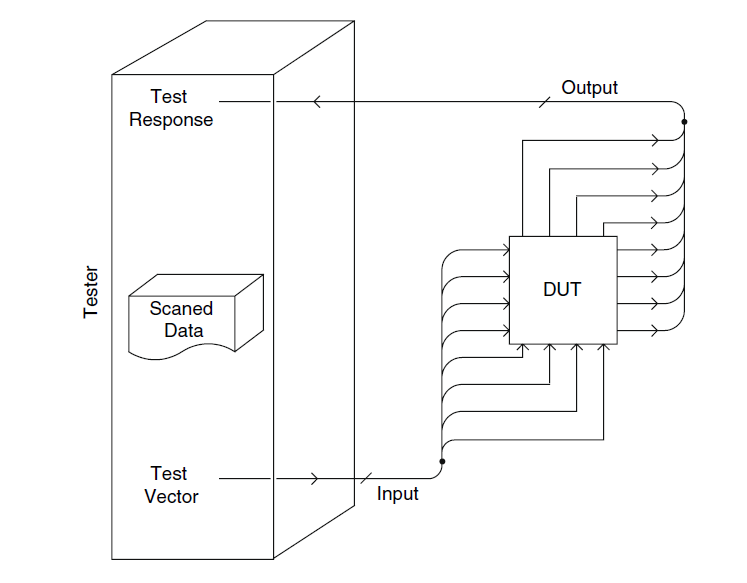
\includegraphics[width=0.65\textwidth]{figures/test.png}
\caption{The tester principle~\cite{book:Navabi}}
\label{fig:test}
\end{figure}

The tester is responsible for test vector generation, feeding the vectors to the inputs of the Device Under Test (DUT), gathering the response and evaluating it. Both generation and evaluation tasks are very design dependent and have to be adjusted after the design is placed in the test bench. The easiest interface from the users perspective is a PC application acting as the GUI. Since the UUT is being developed on the RTL level with hardware description language and the test bench is supposed to test it for real working frequencies, at least as close as possible to real environment, implementation on an FPGA would allow such test. The feeding and gathering has to also be implemented in FPGA as physical test interface. The middleware, responsible for the communication and translation of signals, should support standard communication protocols for data exchange with PC and hardware interface to the FPGA. The rough design draft is shown in the figure \autoref{fig:draft}.\\
 

\begin{figure}[H]
\centering
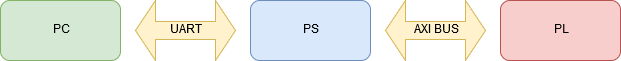
\includegraphics[width=0.65\textwidth]{figures/PCPSPL.png}
\caption{Draft of the test system}
\label{fig:draft}
\end{figure}

\section {Target Architecture}
The target architecture chosen is the Xilinx Zynq SoC (system on Chip). The idea of integrating processors, memories, mixed signal components with RF components in one chip has been known for a long time. Such Application Specific Integrated Circuits (ASICs) are designed to reduce size, to target more secure and faster communication between systems, to lower power consumption and increase reliability. The production cost of a single ASIC is also lower. The main problem of such full custom design is lack of flexibility, high, non-recurring development cost and time. Another important drawback is the lack of compatibility with most of standard applications which speed up the development process and, what comes with it, the time to market. Instead of full-custom ASICs, the semi custom SoCs with programmable logic are gaining on importance. Standard processors connected with Field Programmable Arrays (FPGAs), peripherlas and communication systems create an All-Pogrammable-System-on-Chip. The Programmable Logic is ideal for implementing high-speed logic and data flow systems, while Processing System supports operating system and standard software routines.The combination allows the developer to apply any system and easily partition it between hardware and software.

The Xilinx Zynq XC7Z020-1-CLG484 produced in 28nm technology is a SoC solution containing an ARM hardware processor with two cores and an FPGA with 53200 LUTs, 106400 DFFs and 560 KB of Block RAM. It supports all common standard communication interfaces: UART, SPI, CAN, I2C, GigE, GPIO and SDIO . It also allows quick data transfers between Pocessing System (PS) and Programmable Logic (PL) thanks to Xilinx AXI Bus. The full overview of the Zynq architecture is shown in \autoref{fig:Zynq}. The platform suits all needs of the hardware and middleware layer of the test bench.

\begin{figure}[H]
\centering
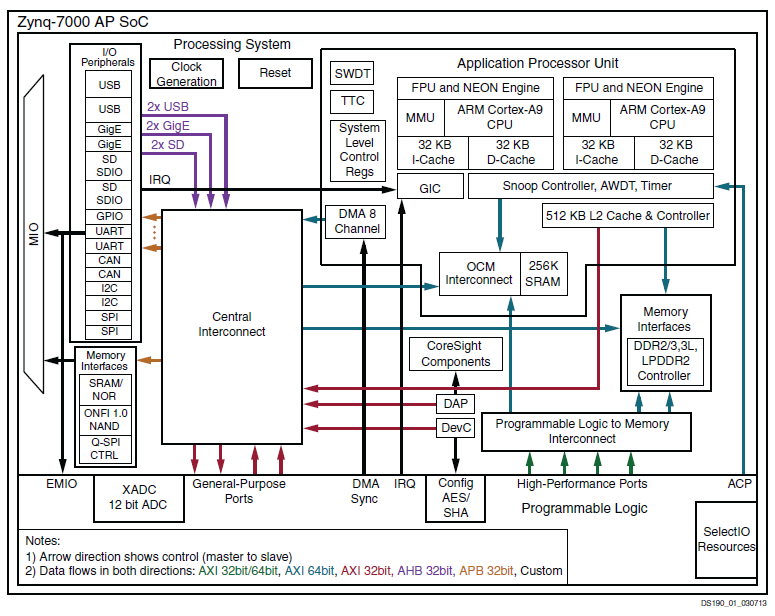
\includegraphics[width=0.65\textwidth]{figures/Zynq.png}
\caption{The Zynq Processing System~\cite{book:ZynqBook}}
\label{fig:Zynq}
\end{figure}

\section{Physical Interface}
The physical interface of the test bench has to supply UUT inputs with test vectors and record response of the outputs. This is the principle of the boundary test, where the tester has no access to the internal structure of the tested design. The system architecture is shown in \autoref{fig:testbench}.

\begin{figure}[H]
\centering
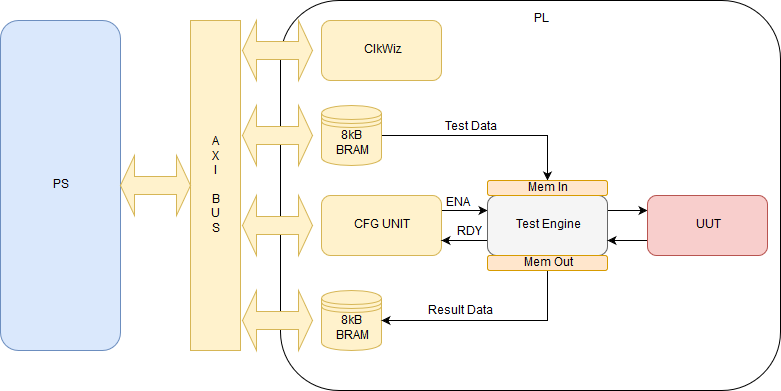
\includegraphics[width=0.65\textwidth]{figures/TestBench.png}
\caption{The Architecture of the Test Bench~\cite{book:ZynqBook}}
\label{fig:testbench}
\end{figure}

\subsection{AXI Interface}
The history of the Advanced eXtensible Interface (AXI) goes back to year 2003 when it was first introduced as part of the ARM\textsuperscript{\textregistered} Advanced Microcontroller Bus Architecture (AMBA\textsuperscript{\textregistered}). The current version is called AXI4 and was released in 2010 as second version of AXI interface. The number four comes from the fourth version of AMBA, which contains AXI interface. The protocol is supported by many Intellectual Property (IP) producers (not only Xilinx) making the designer learn only one standard of communication. It was developed to standardize the communication between modules in the SoC designs. There are three types or modes of the AXI4:
\begin{itemize}
    \item AXI4 maps the memory of the interface and allows bursts up to 256 data transfers with just single address phase. Writing data to the memory, sends the data directly to the IP,
    \item AXI4-Lite is a light-weight version which offers just memory mapping without the burst capability,
    \item AXI4-Stream doesn't support any address phases. It allows unlimited burst of data. Lack of addresses make it no more considered a memory mapping interface.
\end{itemize}
The protocol works in the master slave system connecting both of them using an AXI Interconnect IP. It applies only to memory mapped versions, since the AXI4-Stream connects master and slave directly or with each other or DMA IP. The AXI Interconnect can service up to 16 masters and 16 slaves. Its main function is the data-width translation, downsizing too big master data packets into smaller slave-compliant bursts or upsizing it. It also does the clock-rate conversion, since both masters and slaves can operate on different clock frequencies. One of the big advantages of the interconnection is the mix support between protocol modes. Moreover the interconnection implements data pipelining for better frequency vs. latency trade-off. Finally it handles priorities in data transitions, making them either concurrent or using programmable priorities.
AXI4 protocol is designed for bidirectional communication, having separate write address, read address, write data, read data and write response channels in memory mapped modes and just data transfer channel in Stream mode. Every Xilinx IP has AXI4 support and there is an easy way of creating custom IPs supporting this protocol~\cite{report:AXI}.

\subsection{Test Engine}\label{ssec:engine}
The main core of the Test Bench is the Test Engine which feeds the test vectors to the UUT and gathers the response vectors. It consist of two parts:
\begin{itemize}
    \item memory interface which calculates successive addresses for words in the memory bank and stores them in the input register for one $clk_{bram}$ cycle. The addresses get incremented by $inc = width_{bram}/8$ due to the bytewise addressing scheme. The memory interface also handles the write back of the response once per $clk_{bram}$ cycle from the output register. The number of pipeline stages for data read operation has to be taken into account. The number of pipeline stages determines the delay in clock cycles when the information, stored under the address given in the address register, actually gets to the input register of the test engine. The detailed timing is showed in \autoref{fig:timing}.
    \item data downsize converter which reads input register and conducts parallel to parallel conversion where the input dimension is the $b=width_{bram}$ and the output dimension is the $u=width_{uut}$. The conversion process takes $k clk_{uut}$ cycles where $k$ is calculated as showed in~\autoref{eq:ratio}.
    \begin{equation}\label{eq:ratio}
    k = \frac{clk_{uut}}{clk_{bram}} = \frac{width_{bram}}{width_{uut}}
    \end{equation}
    The Test Engine successively shifts the $u$ size chunks of data through the design. With each $clk_{uut}$ cycle new data is placed on the input of UUT and new response gathered. The upsize converter recombines the $u$ size responses into $b$ size word with another parallel to parallel conversion. The test vector and response vector have always the same width $u$, although the number of UUT inputs and outputs may vary. It is necessary to connect the unused ports of the Test Engine to a known constant value.
\end{itemize}
The downsize conversion can be accomplished using a big multiplexer, which $b$ number of inputs and $u$ number of outputs. The multiplexing can be also achieved with 8 k-to-1 MUXes, which is how the synthesis tool in Vivado handles this problem. The multiplexer solution is show in \autoref{fig:mux}.

Another way of conducting a donwsize conversion is by splitting it to many parallel to serial conversions. Such conversions are done using shift registers with parallel inputs but serial outputs.

\begin{figure}[h]
\centering
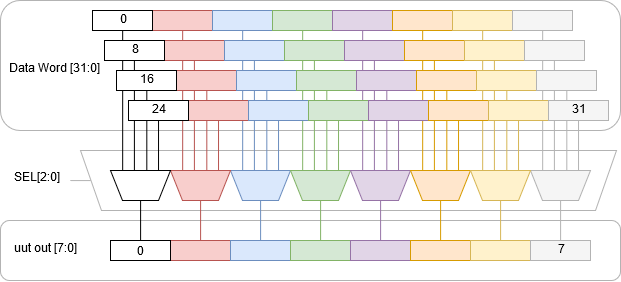
\includegraphics[width=0.65\textwidth]{figures/MUX.png}
\caption{MUX}
\label{fig:mux}
\end{figure}

\begin{figure}[h]
\centering
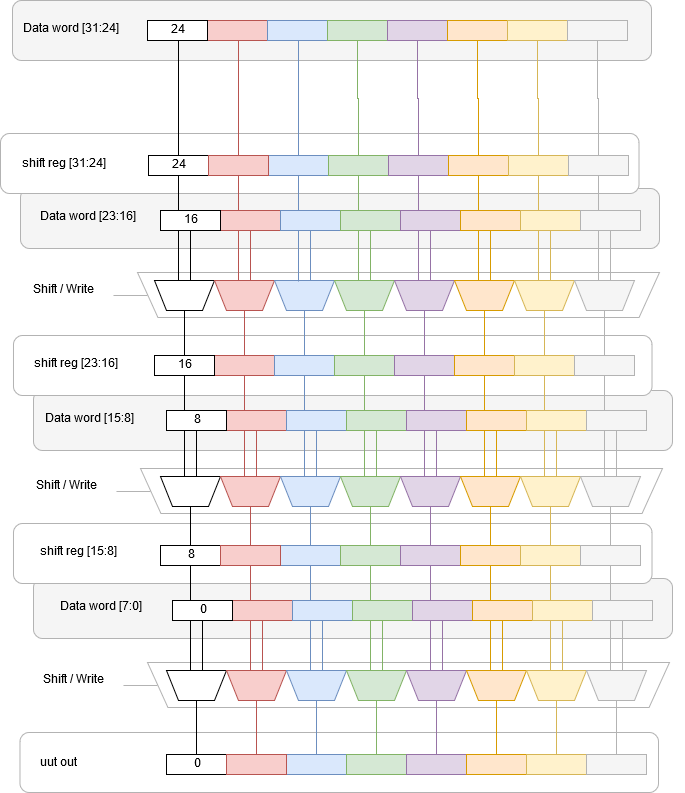
\includegraphics[width=0.65\textwidth]{figures/Shift_2.png}
\caption{Shift register}
\label{fig:shift}
\end{figure}
%---!!!! see how it is implemented and repair!!!!!---%%%
The UUT is surrounded by flip-flops to guaranty, that the tested design is separated from the test engine logic.
\subsection{Data buffering}
Since the test has to be conducted with working frequency of the design, the data fed to the test bench has to be buffered. Working with the native AXI frequency of 200 MHz and providing the clock signal as one of the data bits would result in the maximum test frequency being 100Mhz. Buffering limits the amount of data processed during one test run. After all data have been processed, the execution stops and doesn't restart until new data has been written to the memory. For the buffering, the internal Block RAMs have been used. Since they have dual port access, they fit perfectly for the scenario. The dual port capability of a memory implementation means concurrent access to the memory bank from two independent sources. They can be even clocked with two different clocks if necessary. The conflicts, when accessing the IP over AXI4, are handled by the interconnect which schedules the write and read access after each other. In the true dual port configuration, whithout the AXI4 protocol, the conflict management can be configured, but conflicts are advised to be avoided~\cite{report:BRAM}.

The BRAMs in the test bench are configured to be true dual ports. One port connected to AXI Bus and another port to the Test Engine. Conflicts must never occur because of the state machine implemented. The memory is never accessed by PL and PS simultaneously. The state machine is shown in the \autoref{fig:PSschedule}. There are two instances of the BRAMs, one to supply the stimuli to the Test Engine, another to store responses. The input BRAM is filled with data. Then the ENA signal starts the test procedure, resulting in: valid responses stored in output BRAM and RDY signal, to indicate the end of the test procedure. The lack of simultaneous accesses from PL and PS allows the use of only one BRAM, connecting one port as the input to the Test Engine and another port as its output. After the test routine ends, it would be possible to switch the connection of one of the ports back to the AXI interface. This solution is more area efficient, but the presence of two BRAMS was determined by a possible extra feature of conducting successive runs with the same stimuli or chaining the output BRAM to be the input of another Test Engine. 

The depth and width of the BRAMs may be adjusted to suit the testers needs and optimize BRAMs function. They have to be kept equal for both BRAMs at all times. The width of the memory is a very important parameter for frequency multiplication. The $clk_{bram}$ is different then the $clk_{uut}$ and their relation $k$ is strongly connected with the width of BRAM word and the width of the UUT interface showed in~\autoref{eq:ratio}. For example if the $width_{uut} = 8b$ and the desired test frequency set to $clk_{uut} = 300MHz$ and the BRAM configured to have $width_{bram} = 16b$ then it would have to be clocked with the frequency $clk_{bram} = 150MHz$ to satisfy data throughput. It usually makes sense to set the $width_{bram} > width_{uut}$ to access frequncies higher then $clk_{bram_{max}} = 400 MHz$. The detailed explanation of the origin of this relation can be found in \autoref{ssec:engine}.


\section{Middleware}
\section{GUI}